% !TeX root = ../main.tex

% \begin{frame}
%   \frametitle{Relative Homology and The TCC}
%
%   \begin{itemize}
%     \item Relative homology and separation,
%     \item Properties of surrounding pairs,
%     \item Assumption 1 and The Geometric TCC,
%     \item Duality, Assumption 2, and the Algorithmic TCC.
%   \end{itemize}
% \end{frame}

\begin{frame}
  \frametitle{Relative Homology and Separation}

  \begin{textblock*}{10cm}(1cm,4.5cm)
    \centering
    \includegraphics<1,2>[width=\textwidth]{figures/h1_rel}
    \includegraphics<2>[width=\textwidth]{figures/h2_rel}
  \end{textblock*}

\end{frame}

\begin{frame}
  \frametitle{Properties of Surrounding pairs}

  \begin{textblock*}{11cm}(1cm,2cm)
    \begin{small}
      \only{Surrounding pair $(D, B)$, }
      \only<2,3>{complement $(\overline{B}, \overline{D})$.\vspace{1ex}}

      \only<3>{$D\setminus B$ and $\overline{D}$ disconnected $\implies \hom_k(D\setminus B)\cong\hom_k(\overline{B},\overline{D})$.}

    %   \begin{lemma}\label{lem:coverage}
    %     If $\ell$ is injective then $D\setminus B_\omega\subseteq P^\delta$ and $Q_0^\delta$ surrounds $P^\delta$ in $D$.
    %   \end{lemma}
    % \end{small}
    \end{small}
  \end{textblock*}

  \begin{textblock*}{12cm}(0.75cm,5cm)
    \includegraphics<1,2>[trim=50 250 50 300, clip, width=0.4\textwidth]{figures/comp/surf}
    \includegraphics<3>[trim=50 250 50 300, clip, width=0.4\textwidth]{figures/comp/Bint}\only<2,3>{\hspace{6ex}}
    \includegraphics<2,3>[trim=50 250 50 300, clip, width=0.4\textwidth]{figures/comp/DBcomp}
  \end{textblock*}
\end{frame}

\begin{frame}
  \frametitle{Properties of Surrounding pairs}

  \begin{textblock*}{11cm}(1cm,2cm)
    \begin{small}
      Surrounding pair $(D, B)$.\vspace{1ex}

      \only<2,3>{Pair $(U, V)$ with $U\subseteq D$, $V\subseteq U\cap B$.\vspace{1ex}}

      \only<3>{Let $\ell : \hom_0(\overline{B}, \overline{D})\to \hom_0(\overline{V}, \overline{U})$}

    %   \begin{lemma}\label{lem:coverage}
    %     If $\ell$ is injective then $D\setminus B_\omega\subseteq P^\delta$ and $Q_0^\delta$ surrounds $P^\delta$ in $D$.
    %   \end{lemma}
    % \end{small}
    \end{small}
  \end{textblock*}

  \begin{textblock*}{12cm}(0.75cm,5cm)
    \includegraphics<1,2>[trim=50 250 50 300, clip, width=0.4\textwidth]{figures/comp/surf}\only<2>{\hspace{6ex}}
    \includegraphics<2>[trim=50 250 50 300, clip, width=0.4\textwidth]{figures/comp/PQ}
    \includegraphics<3>[trim=50 250 50 300, clip, width=0.4\textwidth]{figures/comp/DBcomp}\only<3>{\hspace{6ex}}
    \includegraphics<3>[trim=50 250 50 300, clip, width=0.4\textwidth]{figures/comp/PQcomp}
    % \includegraphics<4>[trim=50 250 50 300, clip, width=0.4\textwidth]{figures/comp/Bint}\only<4>{\hspace{6ex}}
    % \includegraphics<4>[trim=50 250 50 300, clip, width=0.4\textwidth]{figures/comp/Qint}
    % \includegraphics<2>[trim=50 200 50 200, clip, width=0.45\textwidth]{figures/nbhd/P}
    % \includegraphics<3>[trim=50 200 50 200, clip, width=0.45\textwidth]{figures/nbhd/NP0}
    % \includegraphics<3>[trim=50 200 50 200, clip, width=0.45\textwidth]{figures/nbhd/NP1}
  \end{textblock*}
\end{frame}

\begin{frame}
  \frametitle{Properties of Surrounding pairs}

  \begin{textblock*}{11cm}(1cm,2cm)
    \begin{small}
      \begin{lemma}\label{lem:coverage}
        If $\ell$ is injective then $D\setminus B\subseteq U$ and $V$ surrounds $U$ in $D$.
      \end{lemma}
    \end{small}

  \end{textblock*}

  \begin{textblock*}{12cm}(0.75cm,5cm)
    \includegraphics<1>[trim=50 250 50 300, clip, width=0.4\textwidth]{figures/comp/DBcomp}\only<1>{\hspace{6ex}}
    \includegraphics<1>[trim=50 250 50 300, clip, width=0.4\textwidth]{figures/comp/PQcomp}
    \includegraphics<2>[trim=50 250 50 300, clip, width=0.4\textwidth]{figures/comp/surf}\only<2>{\hspace{6ex}}
    \includegraphics<2>[trim=50 250 50 300, clip, width=0.4\textwidth]{figures/comp/PQnocov}
    \includegraphics<3,4>[trim=50 250 50 300, clip, width=0.4\textwidth]{figures/comp/DBcomp}\only<3,4>{\hspace{6ex}}
    \includegraphics<3>[trim=50 250 50 300, clip, width=0.4\textwidth]{figures/comp/PQnocov_comp}
    \includegraphics<4>[trim=50 250 50 300, clip, width=0.4\textwidth]{figures/comp/PQnocov_comp-spread}
    \includegraphics<5>[trim=50 250 50 300, clip, width=0.4\textwidth]{figures/comp/Bint}\only<5>{\hspace{6ex}}
    \includegraphics<5>[trim=50 250 50 300, clip, width=0.4\textwidth]{figures/comp/Qno_int}


  \end{textblock*}
\end{frame}

\begin{frame}
  \frametitle{Properties of Surrounding pairs}

  \begin{textblock*}{11cm}(1cm,2cm)
    \begin{small}
      \begin{lemma}\label{lem:coverage}
        If $\ell$ is injective then $D\setminus B\subseteq U$ and $V$ surrounds $U$ in $D$.
      \end{lemma}
    \end{small}

  \end{textblock*}

  \begin{textblock*}{12cm}(0.75cm,5cm)
    \includegraphics<1>[trim=50 250 50 300, clip, width=0.4\textwidth]{figures/comp/surf}\only<1>{\hspace{6ex}}
    \includegraphics<1>[trim=50 250 50 300, clip, width=0.4\textwidth]{figures/comp/PQnosur}
    \includegraphics<2,3>[trim=50 250 50 300, clip, width=0.4\textwidth]{figures/comp/DBcomp}\only<2,3>{\hspace{6ex}}
    \includegraphics<2>[trim=50 250 50 300, clip, width=0.4\textwidth]{figures/comp/PQnosur_comp}
    \includegraphics<3>[trim=50 250 50 300, clip, width=0.4\textwidth]{figures/comp/PQnosur_comp-spread}
    \includegraphics<4>[trim=50 250 50 300, clip, width=0.4\textwidth]{figures/comp/Bint}\only<4>{\hspace{6ex}}
    \includegraphics<4>[trim=50 250 50 300, clip, width=0.4\textwidth]{figures/comp/Qno_int}

  \end{textblock*}

  % \begin{textblock*}{10cm}(0.5cm,5cm)
  %   \only<6>{\begin{description}
  %       \item[Goal:] Show
  %         \[ \ell : \hom_0(\overline{B_\omega}, \overline{D})\to \hom_0(\overline{Q^\delta},\overline{P^\delta})\]
  %         is injective.
  %     \end{description}}
  % \end{textblock*}
\end{frame}


\begin{frame}
  \frametitle{Overview: The Geometric Case}

  \begin{textblock*}{11cm}(1cm,2cm)
    Unknown $c$-Lipschitz function $f : D\to \R$.\vspace{1ex}

    \only<2,3>{Finite sample $P\subset D$ of $f$.\vspace{1ex}}

    \only<3>{Coverage radius $\delta > 0$, covered region $P^\delta$.}
  \end{textblock*}

  \begin{textblock*}{12cm}(0.5cm,5cm)
    \includegraphics<1>[trim=50 200 50 200, clip, width=0.45\textwidth]{figures/nbhd/D}
    \includegraphics<2>[trim=50 200 50 200, clip, width=0.45\textwidth]{figures/nbhd/P}
    \includegraphics<3>[trim=50 200 50 200, clip, width=0.45\textwidth]{figures/nbhd/CP}
    % \includegraphics<3>[trim=50 200 50 200, clip, width=0.45\textwidth]{figures/nbhd/NP1}
  \end{textblock*}
\end{frame}

\begin{frame}
  \frametitle{Overview: The Geometric Case}

  \begin{textblock*}{11cm}(1cm,2cm)
    Sublevel set $B_\omega$ that surrounds $D$.\vspace{1ex}

    \only<2,3>{Sample $Q$ such that $Q^\delta\subseteq B_\omega$\vspace{1ex}}

    \only<3>{For $\zeta \geq \delta$ set $Q = P\cap B_{\omega-c\zeta}$}
  \end{textblock*}

  \begin{textblock*}{12cm}(0.5cm,5cm)
    \includegraphics<1>[trim=50 200 50 200, clip, width=0.45\textwidth]{figures/nbhd/B0}
    \includegraphics<2>[trim=50 200 50 200, clip, width=0.45\textwidth]{figures/nbhd/Q0}
    \includegraphics<3>[trim=50 200 50 200, clip, width=0.45\textwidth]{figures/nbhd/CQ0}
  \end{textblock*}
\end{frame}

\begin{frame}
  \frametitle{Overview: The Geometric Case}
  \begin{textblock*}{11cm}(1cm,2cm)
    \begin{small}
    \begin{description}
      \item[Goal:] Show $\ell : \hom_0(\overline{B}, \overline{D})\to \hom_0(\overline{Q^\delta},\overline{P^\delta})$ is injective
      \item[Method:] Check $\mathbf{dim}~\hom_0(D\setminus B)\leq \mathbf{dim}~\hom_0(\overline{Q^\delta}, \overline{P^\delta})$
      \item[Problem:] Possible $\mathbf{dim}~\hom_0(D\setminus B)\leq \mathbf{dim}~\hom_0(\overline{Q^\delta}, \overline{P^\delta})$ and $\ell$ is not injective.
      \item<7>[Solution:] Choose $Q_0, Q_1\subset P$ such that $\mathbf{dim}~\hom_0(D\setminus B)\geq \mathbf{rk}~\hom_0((\overline{Q_1^\delta}, \overline{P^\delta})\hookrightarrow(\overline{Q_0^\delta}, \overline{P^\delta}))$.
    \end{description}
    \end{small}
  \end{textblock*}

  \begin{textblock*}{12cm}(0.75cm,5.5cm)
    \includegraphics<2>[trim=50 250 50 300, clip, width=0.4\textwidth]{figures/ass1/surf}\only<1>{\hspace{6ex}}
    \includegraphics<3>[trim=50 250 50 300, clip, width=0.4\textwidth]{figures/ass1/full}
    \includegraphics<4,5>[trim=50 250 50 300, clip, width=0.4\textwidth]{figures/ass1/DBcomp}\only<4,5>{\hspace{6ex}}
    \includegraphics<4>[trim=50 250 50 300, clip, width=0.4\textwidth]{figures/ass1/PQcomp}
    \includegraphics<5>[trim=50 250 50 300, clip, width=0.4\textwidth]{figures/ass1/PQcomp-spread}
    \includegraphics<6>[trim=50 250 50 300, clip, width=0.4\textwidth]{figures/ass1/Bint}\only<6>{\hspace{6ex}}
    \includegraphics<6>[trim=50 250 50 300, clip, width=0.4\textwidth]{figures/ass1/Qint}

  \end{textblock*}
\end{frame}

\begin{frame}
  \frametitle{Overview: The Geometric Case}
  \begin{textblock*}{11cm}(1cm,2cm)
  \begin{small}
    Let $Q_0 = P\cap B_{\omega-c\zeta}$ and $Q_1 = P\cap B_{\omega+c\delta}$\vspace{1ex}

    Let $i : \hom_0(\overline{Q_1^\delta}, \overline{P^\delta})\to \hom_0(\overline{Q_0^\delta}, \overline{P^\delta})$.

    \only<2>{\begin{lemma}\label{lem:psurj}
        If $B_\omega$ surrounds $D$ in $\X$ then $\mathbf{dim}~\hom_0(D\setminus B_\omega)\geq \mathbf{rk}~i$.
    \end{lemma}}
  \end{small}
  \end{textblock*}

  \begin{textblock*}{12cm}(0.75cm,5.5cm)
    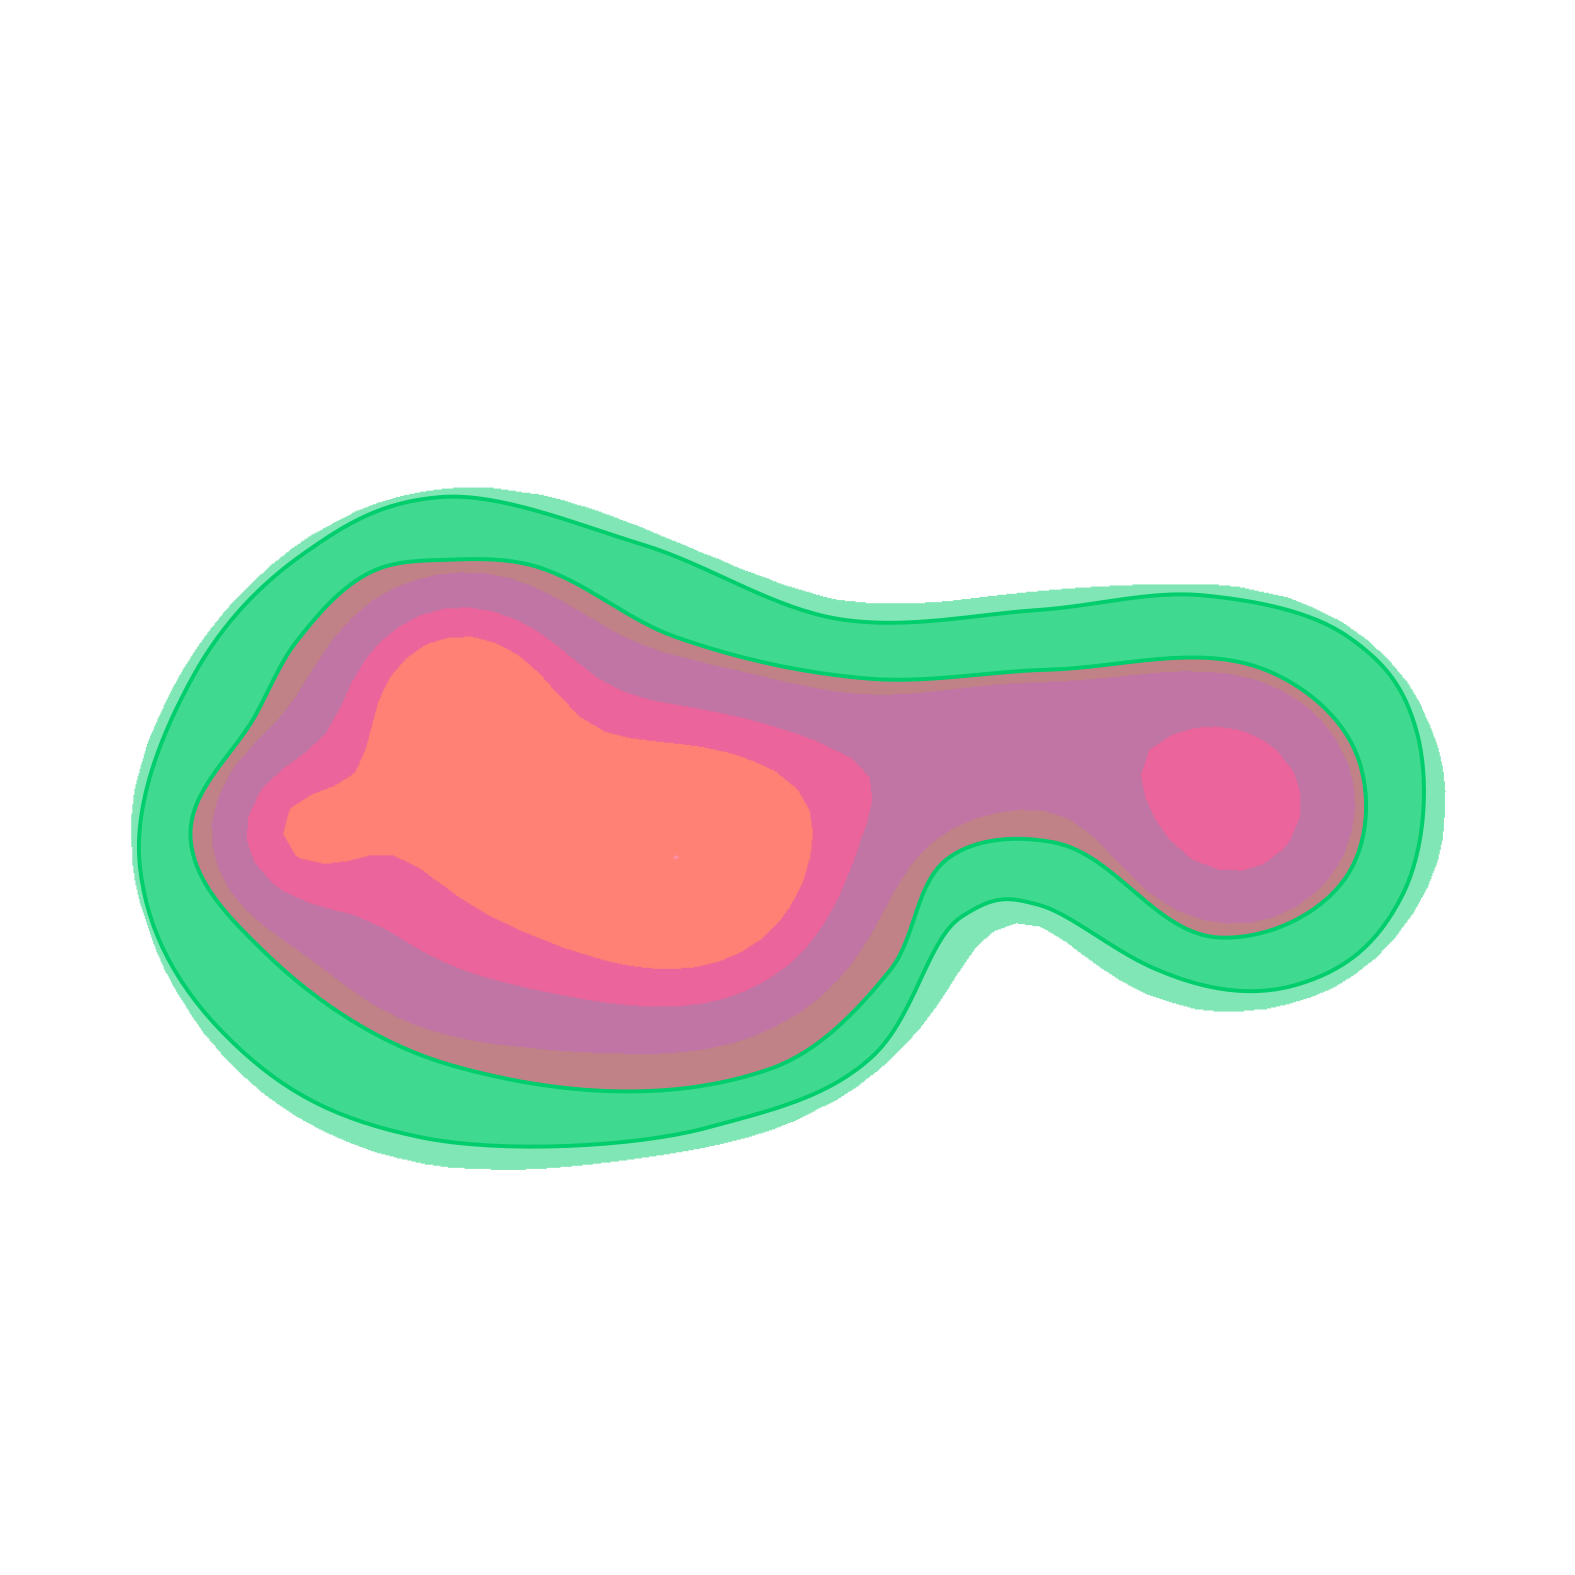
\includegraphics[trim=50 250 50 300, clip, width=0.4\textwidth]{figures/nbhd/PQ0}\hspace{6ex}
    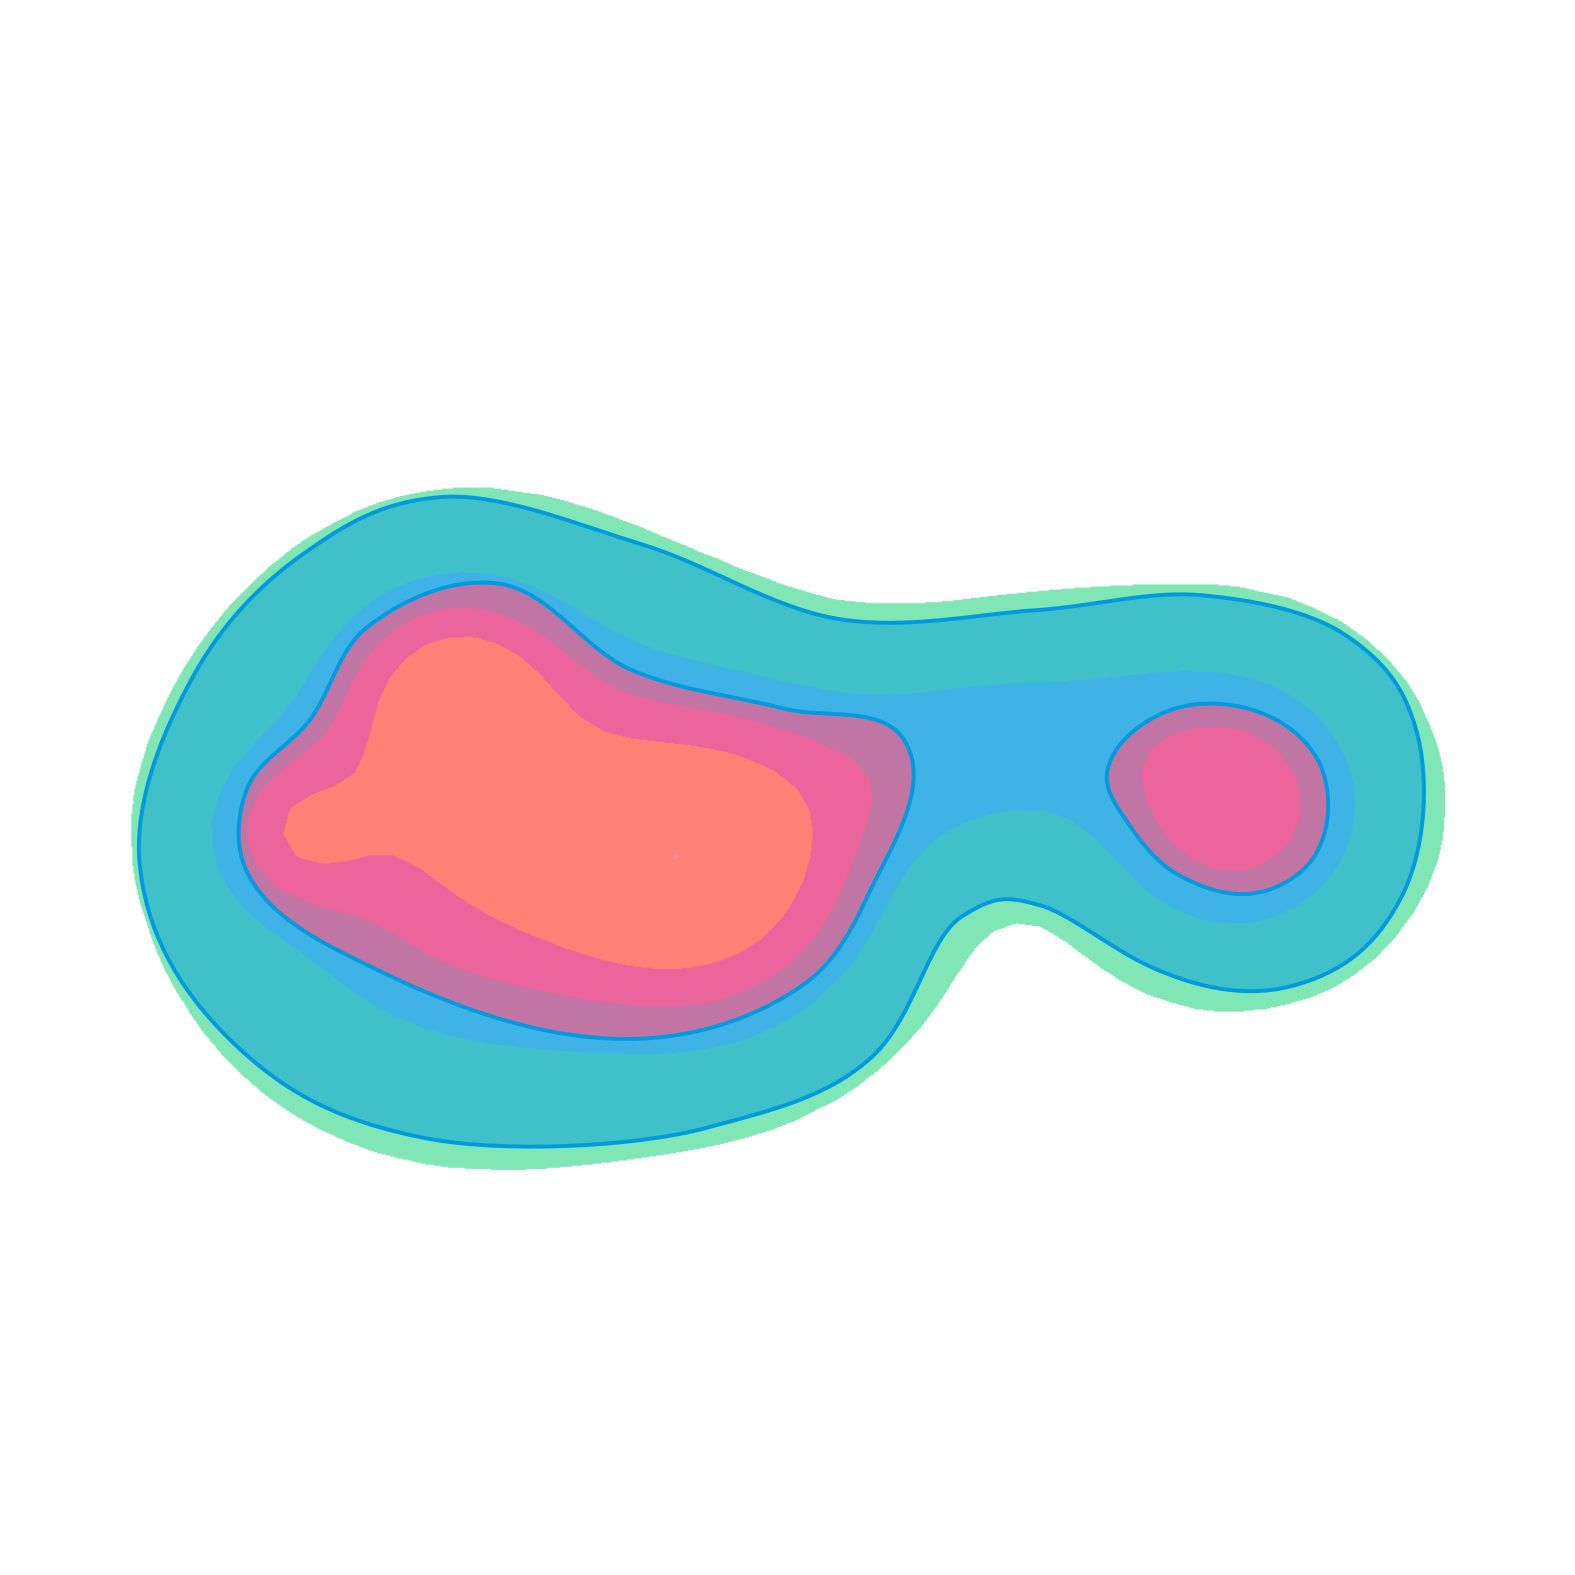
\includegraphics[trim=50 250 50 300, clip, width=0.4\textwidth]{figures/nbhd/PQ1}
  \end{textblock*}
\end{frame}

\begin{frame}
  \frametitle{{\small Assumption 1 and the Geometric TCC}}

  \begin{textblock*}{11cm}(1cm,2cm)
    Recall $\ell$ must be induced by inclusion.\vspace{1ex}

    Let $B_1 = B_{\omega+2c\delta}$ so $Q_1^\delta\subseteq B_1$.\vspace{1ex}
  \end{textblock*}

  \begin{textblock*}{11cm}(1cm,4.5cm)
    \only<1>{\[\begin{tikzcd}[ampersand replacement=\&]
      (P^\delta, Q_0^\delta) \arrow[hookrightarrow]{r}\arrow[hookrightarrow]{d} \&
      (P^\delta, Q_1^\delta) \arrow[hookrightarrow]{d} \\
      %
      (D, B_\omega) \arrow[hookrightarrow]{r} \&
      (D, B_1)
    \end{tikzcd}\]}

    \only<2>{\[\begin{tikzcd}[ampersand replacement=\&]
      \hom_0(\overline{B_1},\overline{D})\arrow{d}{m} \arrow{r}{j} \&
      \hom_0(\overline{B_\omega}, \overline{D}) \arrow{d}{\ell} \\
      %
      \hom_0(\overline{Q_1^\delta}, \overline{P^\delta}) \arrow{r}{i} \&
      \hom_0(\overline{Q_0^\delta}, \overline{P^\delta}).
    \end{tikzcd}\]}
  \end{textblock*}
\end{frame}

\begin{frame}
  \frametitle{{\small Assumption 1 and the Geometric TCC}}

  % \end{tikzcd}\end{equation}
  \begin{textblock*}{11cm}(1cm,2cm)
    \begin{small}
      \begin{description}
        \item[Assumption 1] $j : \hom_0(D\setminus B_{1}\hookrightarrow D\setminus B_\omega)$ is \emph{surjective}.
      \end{description}

      \only<2>{Now, $\mathbf{rk}~j = \mathbf{dim}~\hom_0(D\setminus B_\omega)$.}
    \end{small}
  \end{textblock*}

  \begin{textblock*}{11cm}(1cm,4.5cm)
    % 
\includegraphics[trim=50 190 0 200, clip, scale=0.2]{scripts/figures/scalar.png}
    % 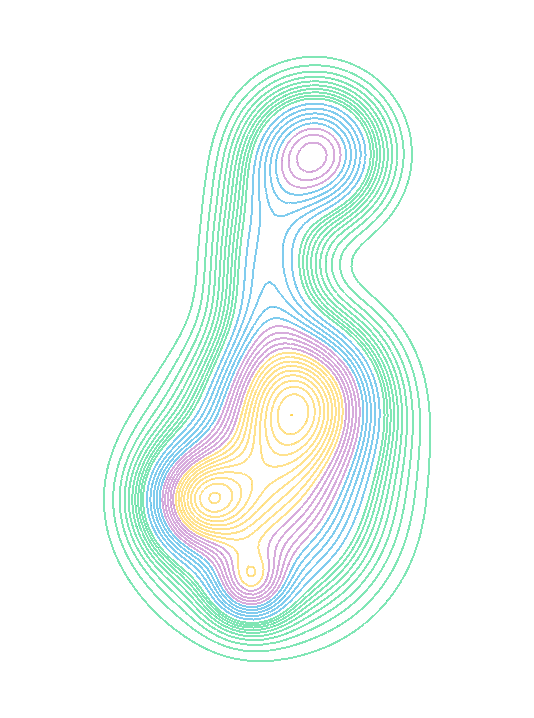
\includegraphics[trim=100 25 75 0, clip, angle=280, scale=0.25]{scripts/figures/scalar_contour.png}
    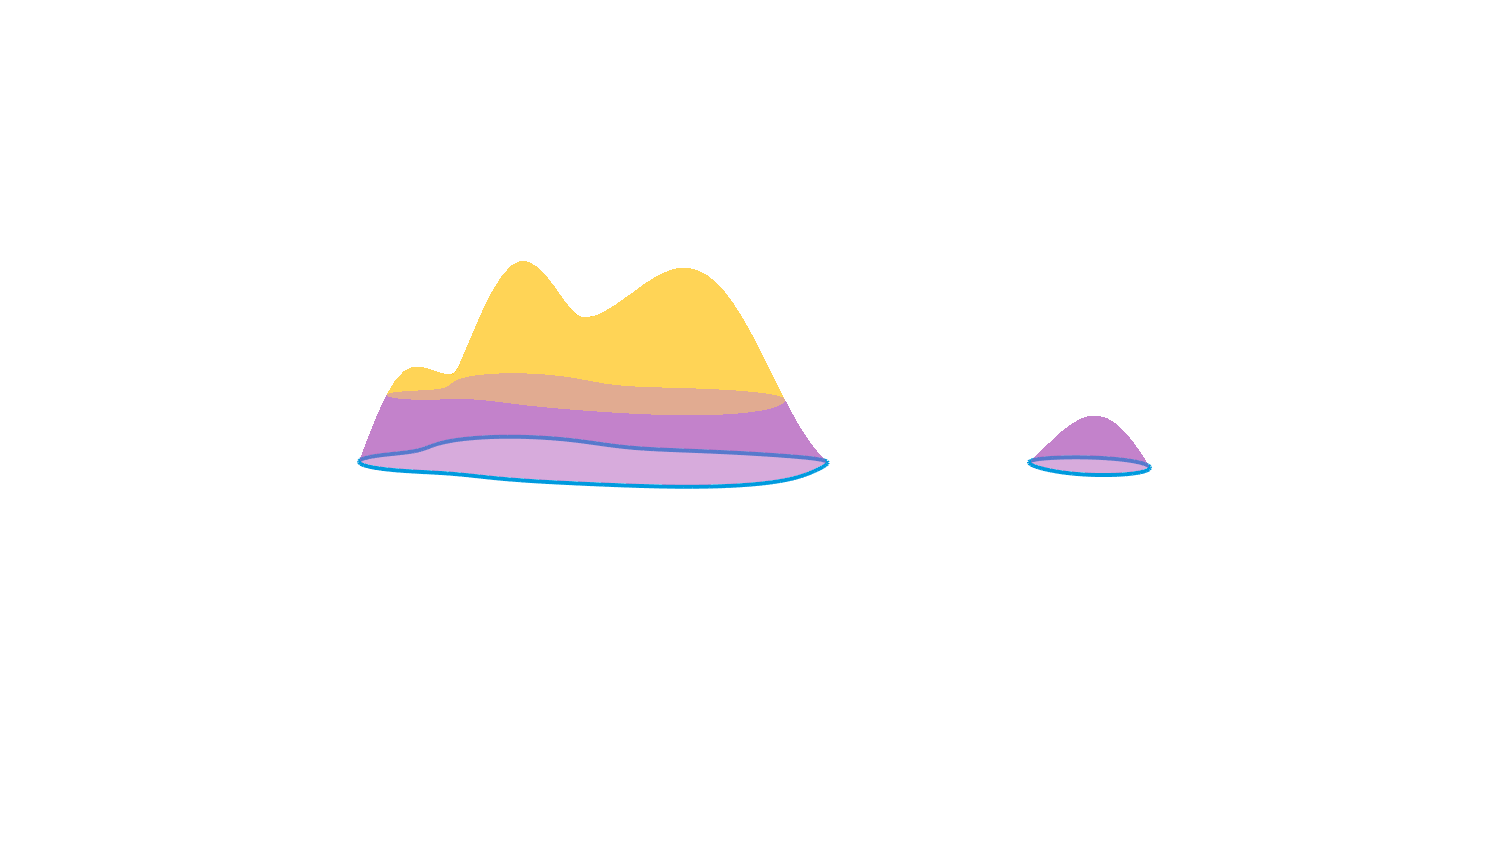
\includegraphics[trim=200 300 200 200, clip, width=0.5\textwidth]{../scripts/figures/surf/ass1_C_side.png}
    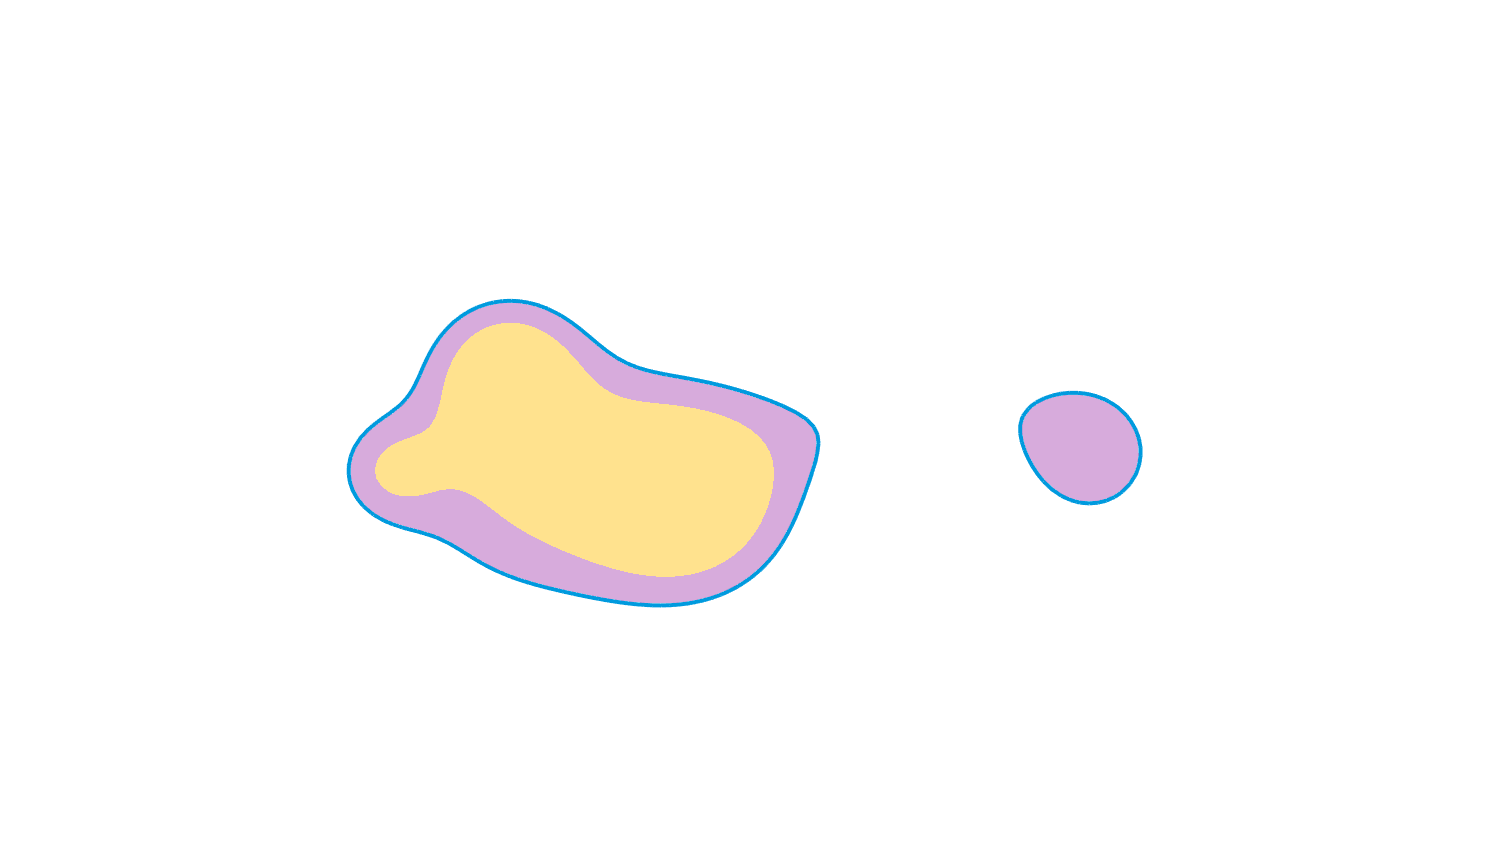
\includegraphics[trim=300 150 200 200, clip, width=0.3\textwidth]{../scripts/figures/surf/ass1_C_top.png}
    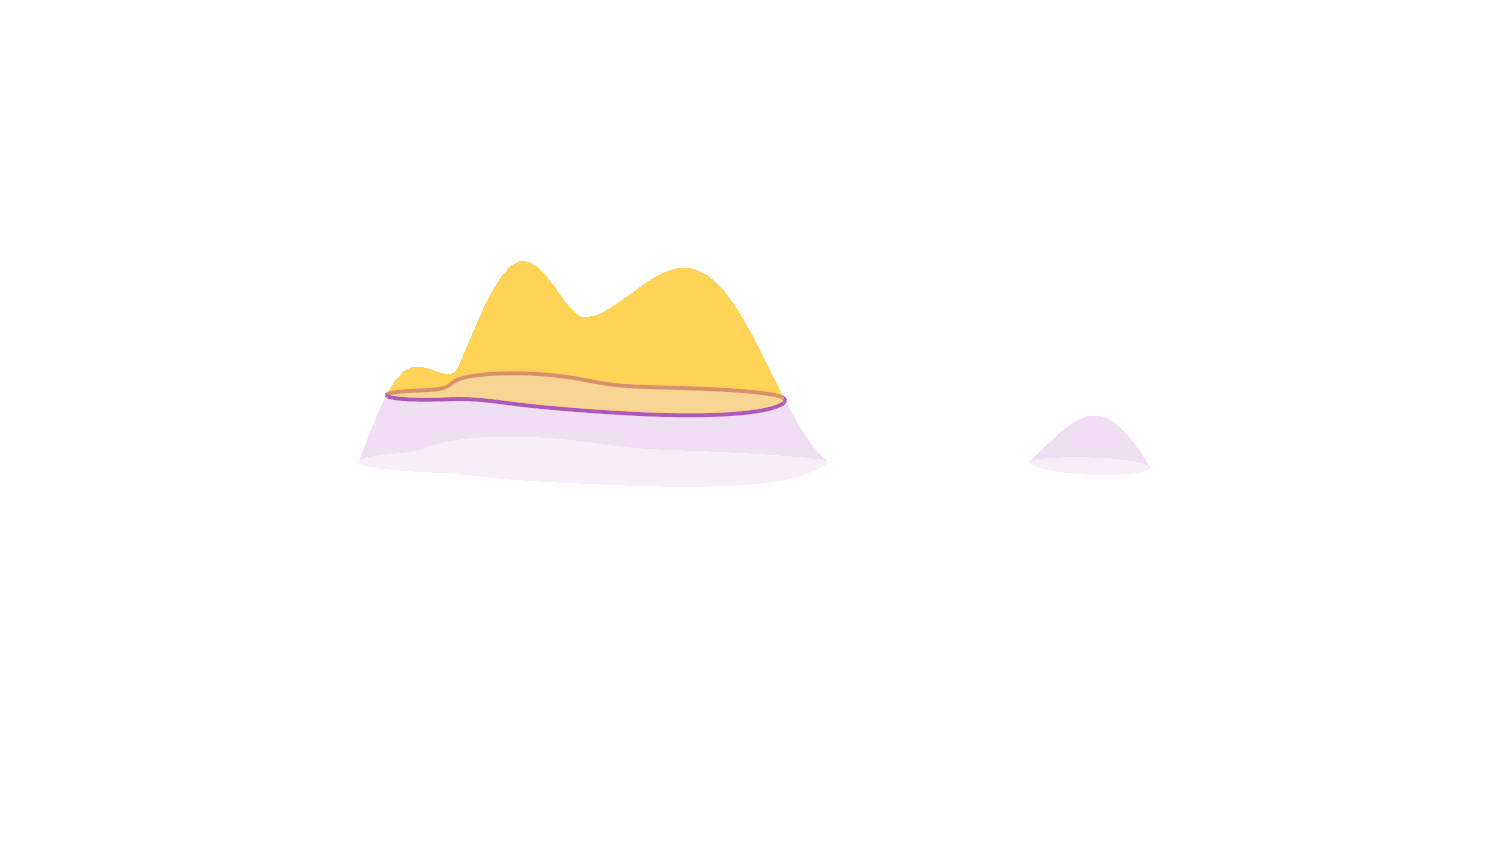
\includegraphics[trim=200 300 200 200, clip, width=0.5\textwidth]{../scripts/figures/surf/ass1_D_side.png}
    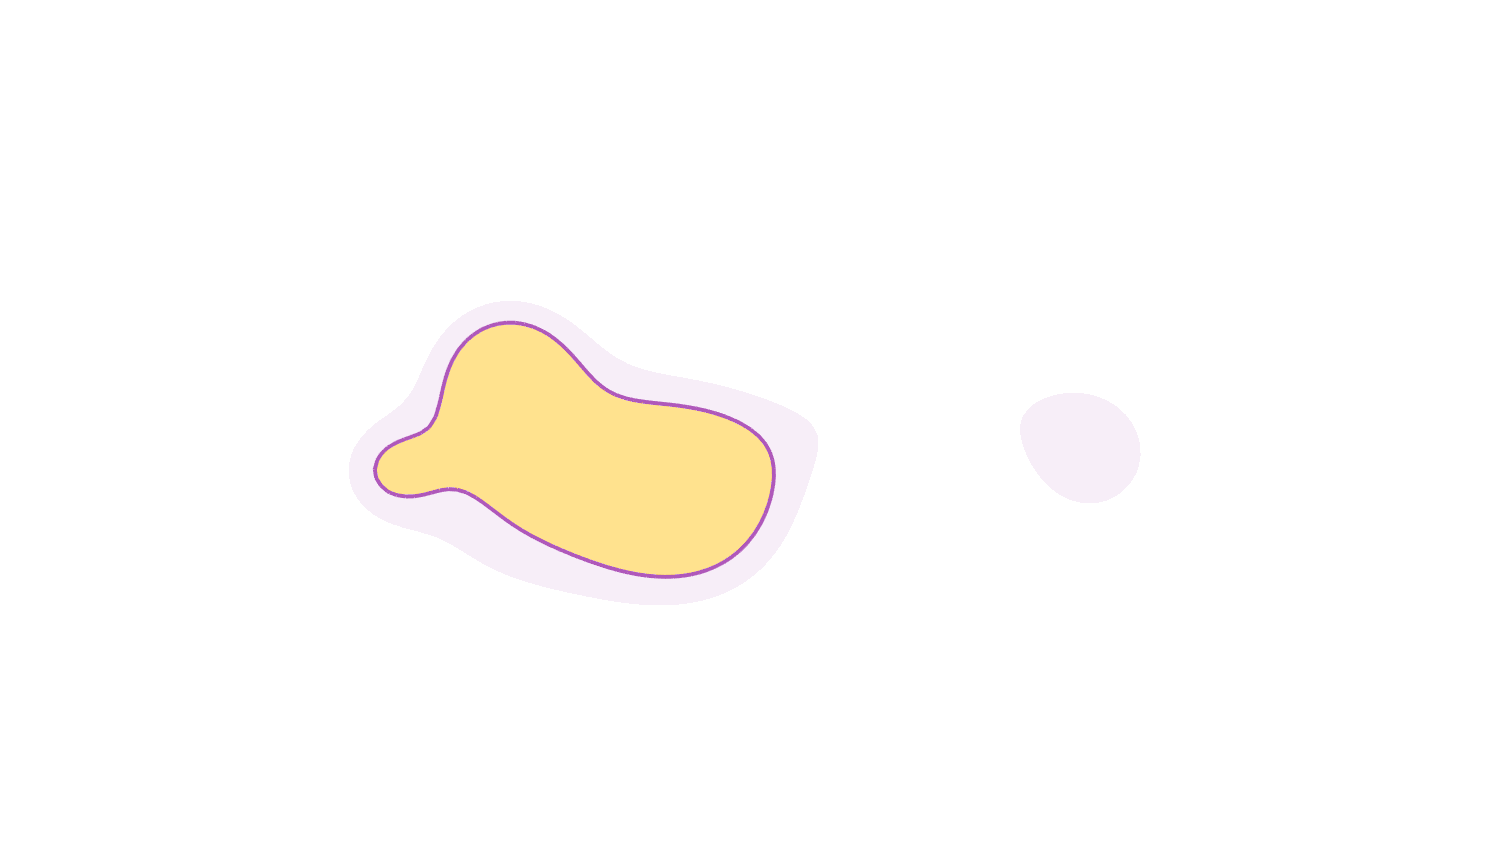
\includegraphics[trim=300 150 200 200, clip, width=0.3\textwidth]{../scripts/figures/surf/ass1_D_top.png}
    % 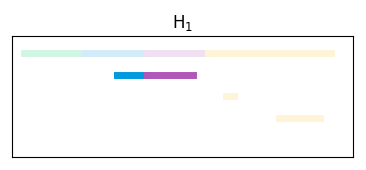
\includegraphics[scale=0.7]{scripts/figures/scalar_barcode_H1-masked.png}
  \end{textblock*}
\end{frame}


\begin{frame}
  \frametitle{{\small Assumption 1 and the Geometric TCC}}

  \begin{textblock*}{11cm}(1cm,2cm)
    \begin{small}\begin{theorem}[Geometric TCC]
        If $j$ is surjective and $\mathbf{rk}~i\geq \mathbf{rk}~j$ then $D\setminus B_\omega\subseteq P^\delta$ and $Q_0^\delta$ surrounds $P^\delta$ in $D$.
    \end{theorem}\end{small}
  \end{textblock*}


  \begin{textblock*}{11cm}(1cm,4.5cm)
    \[\begin{tikzcd}[ampersand replacement=\&]
      \hom_0(\overline{B_1},\overline{D})\arrow{d}{m} \arrow{r}{j} \&
      \hom_0(\overline{B_\omega}, \overline{D}) \arrow{d}{\ell} \\
      %
      \hom_0(\overline{Q_1^\delta}, \overline{P^\delta}) \arrow{r}{i} \&
      \hom_0(\overline{Q_0^\delta}, \overline{P^\delta}).
    \end{tikzcd}\]
  \end{textblock*}
\end{frame}

% \begin{frame}
%   \frametitle{Overview: Main Theorems}
%
%   \begin{textblock*}{11cm}(1cm,2cm)
%     \begin{small}\begin{theorem}[Geometric TCC]
%         If
%         \[ \mathbf{rk}~\hom_0((\overline{Q_1^\delta},\overline{P^\delta})\hookrightarrow (\overline{Q_0^\delta},\overline{P^\delta}))\geq \mathbf{dim}~\hom_0(D\setminus B_\omega)\]
%         then $D\setminus B_\omega\subseteq P^\delta$ and $Q_0^\delta$ surrounds $P^\delta$ in $D$.
%     \end{theorem}\end{small}
%   \end{textblock*}
%
%   \begin{textblock*}{11cm}(1cm,5cm)
%     \only<2>{\begin{small}\begin{theorem}[Algorithmic TCC]
%         If
%         \[ \mathbf{rk}~\hom_d(\rips^\delta(P,Q_0)\hookrightarrow \rips^{2\delta}(P, Q_1))\geq \mathbf{dim}~\hom_0(\rips^\delta(P\setminus Q_{0}))\]
%         then $D\setminus B_\omega\subseteq P^\delta$ and $Q_0^\delta$ surrounds $P^\delta$ in $D$.
%     \end{theorem}\end{small}}
%   \end{textblock*}
%
% \end{frame}

\begin{frame}
  \frametitle{Issues with the Geometric TCC}

  \begin{textblock*}{12cm}(0.5cm,2cm)
    \begin{small}
      \begin{itemize}
        \item Cannot compute the homology of offsets directly.
        \item Do not know $\mathbf{dim}~\hom_0(D\setminus B_\omega)$.
        \item Cannot compute the homology of complements directly.
      \end{itemize}
    \end{small}
  \end{textblock*}

\end{frame}

\begin{frame}
  \frametitle{Overview: Computing the TCC}

  \begin{textblock*}{11cm}(1cm,2cm)
    Unknown $c$-Lipschitz function $f : D\to \R$.\vspace{1ex}

    \only<2,3>{Finite sample $P\subset D$ of $f$.\vspace{1ex}}

    \only<3>{Pair of neighborhood graphs on $P$.}
  \end{textblock*}

  \begin{textblock*}{12cm}(0.5cm,4.5cm)
    \includegraphics<1>[trim=50 200 50 200, clip, width=0.45\textwidth]{figures/nbhd/D}
    \includegraphics<2>[trim=50 200 50 200, clip, width=0.45\textwidth]{figures/nbhd/P}
    \includegraphics<3>[trim=50 200 50 200, clip, width=0.45\textwidth]{figures/nbhd/NP0}
    \includegraphics<3>[trim=50 200 50 200, clip, width=0.45\textwidth]{figures/nbhd/NP1}
  \end{textblock*}
\end{frame}

\begin{frame}
  \frametitle{Overview: Computing the TCC}

  \begin{textblock*}{11cm}(1cm,2cm)
    Sublevel set $B_\omega$ that \emph{surrounds} $D$.\vspace{1ex}

    \only<2,3>{Samples $Q_0, Q_1\subset P$ near $B_\omega$\vspace{1ex}}

    \only<3>{Rips tells us about $(P^\delta, Q_0^\delta)\hookrightarrow (P^\delta, Q_1^\delta)$}
  \end{textblock*}

  \begin{textblock*}{12cm}(0.5cm,5cm)
    \includegraphics<1>[trim=50 200 50 200, clip, width=0.45\textwidth]{figures/nbhd/B0}
    \includegraphics<2>[trim=50 200 50 200, clip, width=0.45\textwidth]{figures/nbhd/NQ0}
    \includegraphics<2>[trim=50 200 50 200, clip, width=0.45\textwidth]{figures/nbhd/NQ1}
    \includegraphics<3>[trim=50 200 50 200, clip, width=0.45\textwidth]{figures/nbhd/PQ0}
    \includegraphics<3>[trim=50 200 50 200, clip, width=0.45\textwidth]{figures/nbhd/PQ1}

  \end{textblock*}
\end{frame}


\begin{frame}
  \frametitle{{\small Assumption 2, Duality, and the Algorithmic TCC}}

  \begin{textblock*}{12cm}(0.5cm,2cm)
    \begin{small}
      \begin{itemize}
        \item Cannot compute the homology of offsets directly.
        \item Do not know $\mathbf{dim}~\hom_0(D\setminus B_\omega)$.
        \item Cannot compute the homology of complements directly.
      \end{itemize}
    \end{small}
  \end{textblock*}

  \begin{textblock*}{12cm}(1cm,5cm)
    \only<2>{Let $B_0\ldots$}
  \end{textblock*}
\end{frame}

\begin{frame}
  \frametitle{{\small Assumption 2, Duality, and the Algorithmic TCC}}

  % \end{tikzcd}\end{equation}
  \begin{textblock*}{11cm}(1cm,2cm)
    \begin{small}
      \only<1>{\begin{description}
        \item[Assumption 2] $\hom_0(D\setminus B_\omega\hookrightarrow D\setminus B_{0})$ is \emph{injective}.
      \end{description}}

      \only<2>{\begin{lemma}\label{lem:assumption2}
        If $\hom_0(D\setminus B_\omega\hookrightarrow D\setminus B_{0})$ is injective then $\mathbf{dim}~\hom_0(\rips^\delta(P\setminus Q_{0})) \geq \mathbf{dim}~\hom_0(D\setminus B_\omega)$.
      \end{lemma}}
    \end{small}
  \end{textblock*}

  \begin{textblock*}{12cm}(1cm,4.5cm)
    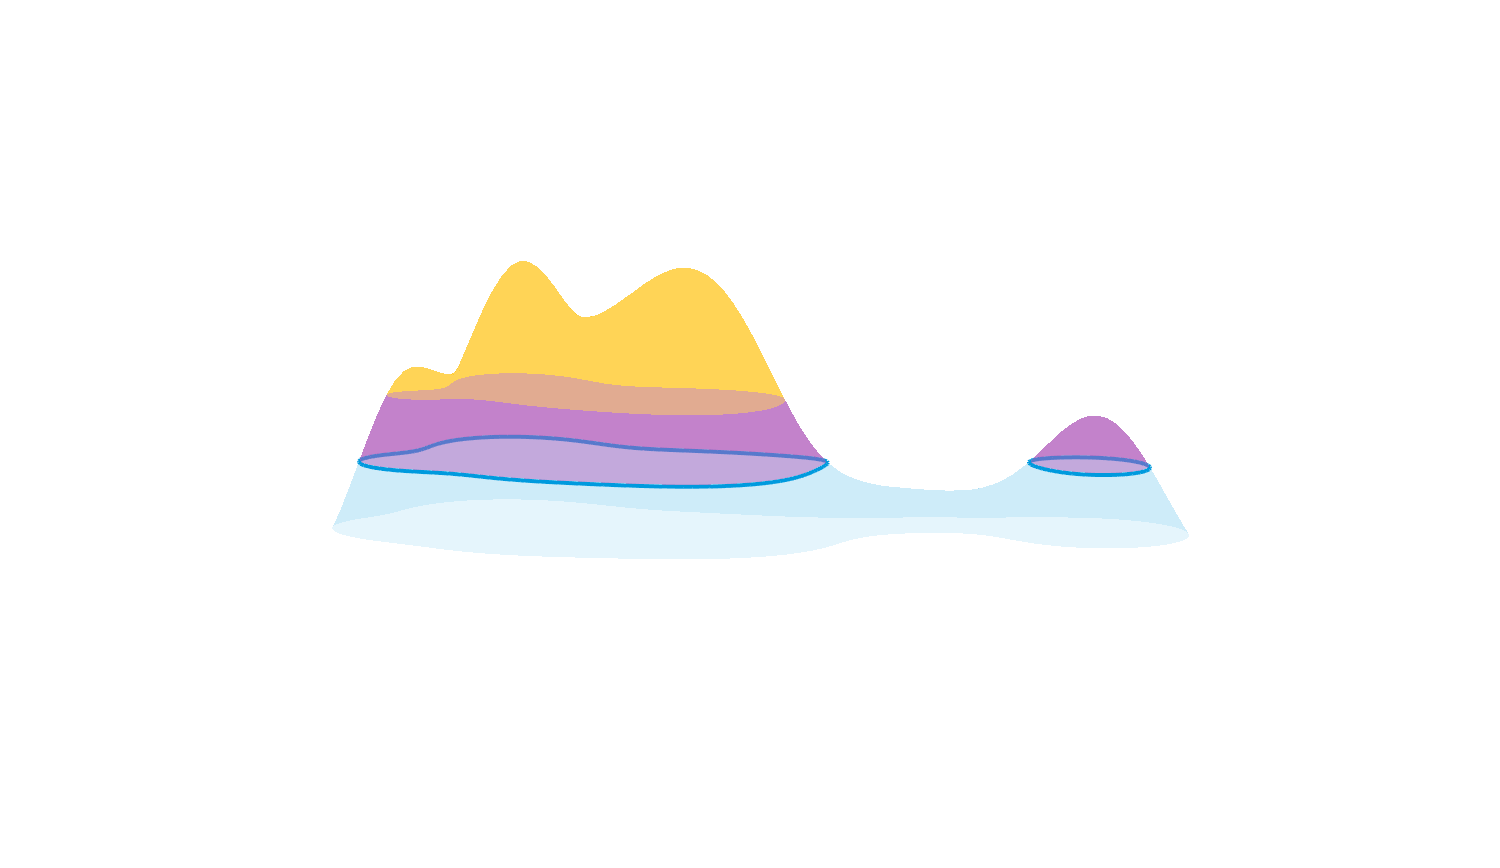
\includegraphics[trim=200 300 200 200, clip, width=0.5\textwidth]{../scripts/figures/surf/ass2_C_side.png}
    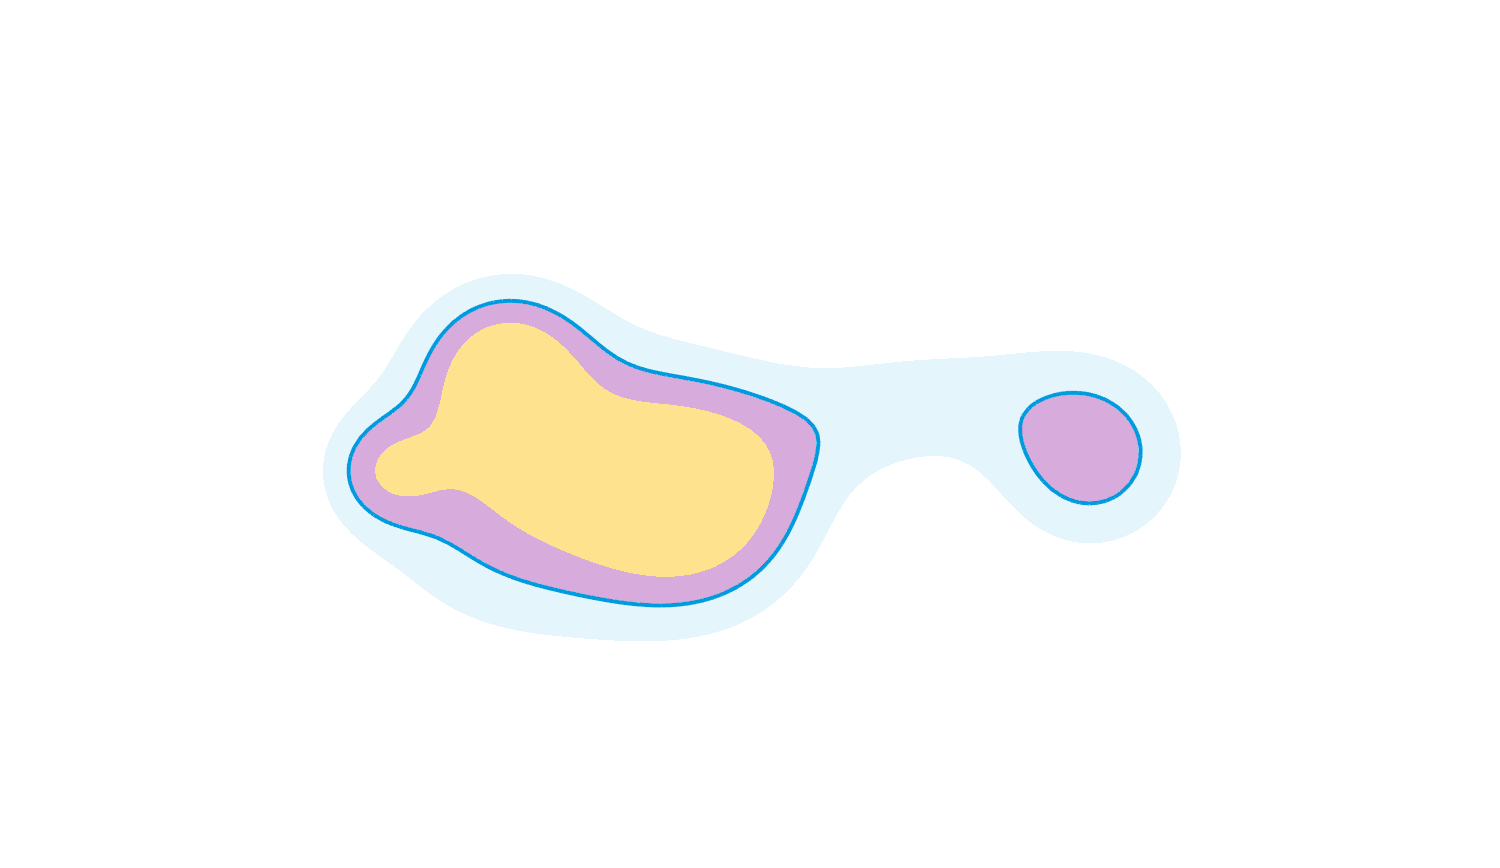
\includegraphics[trim=300 200 200 200, clip, width=0.3\textwidth]{../scripts/figures/surf/ass2_C_top.png}
    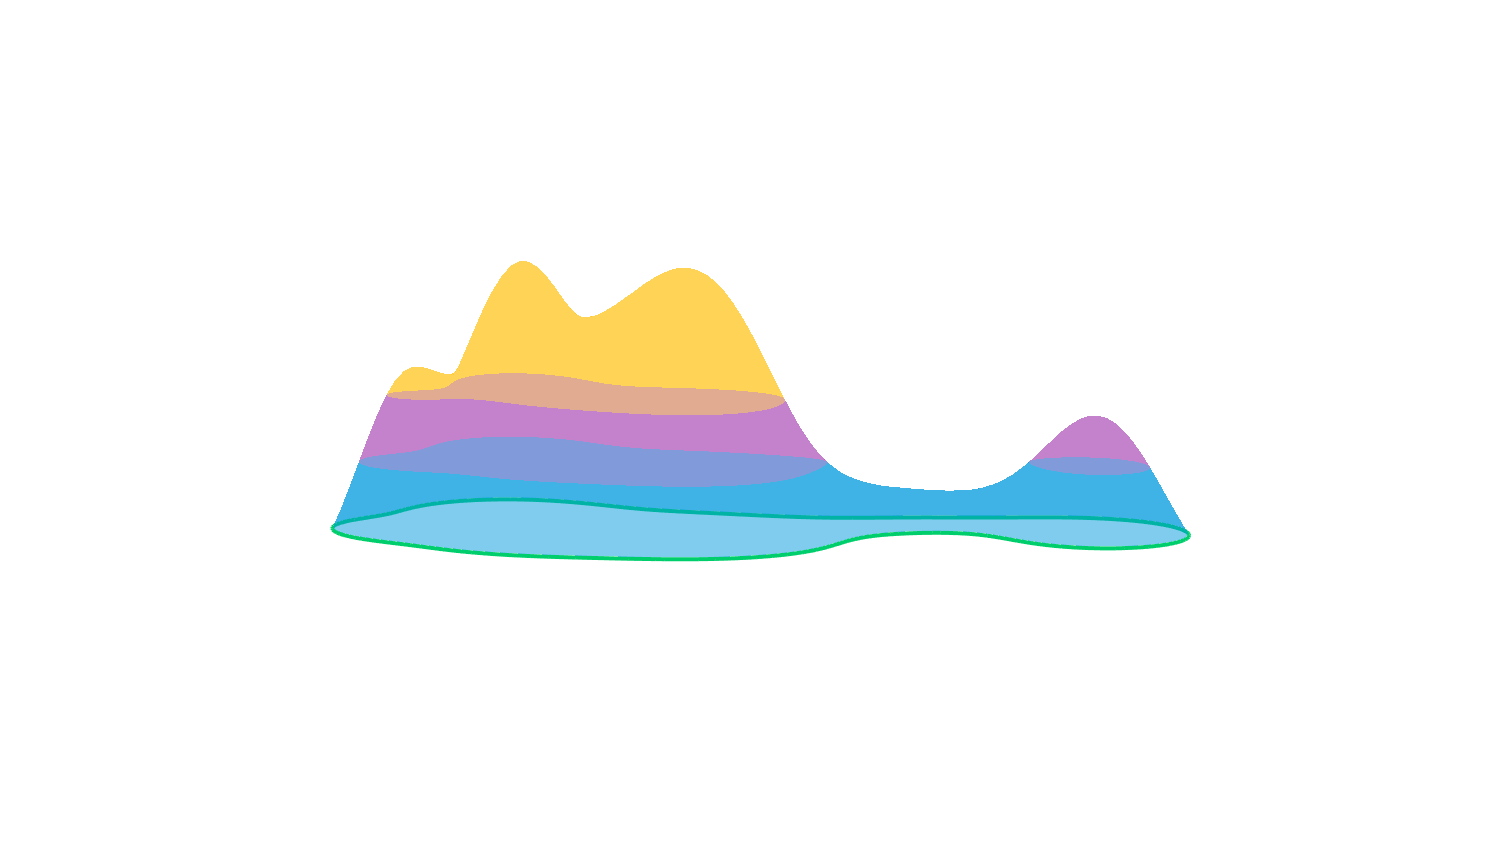
\includegraphics[trim=200 300 200 200, clip, width=0.5\textwidth]{../scripts/figures/surf/ass2_B_side.png}
    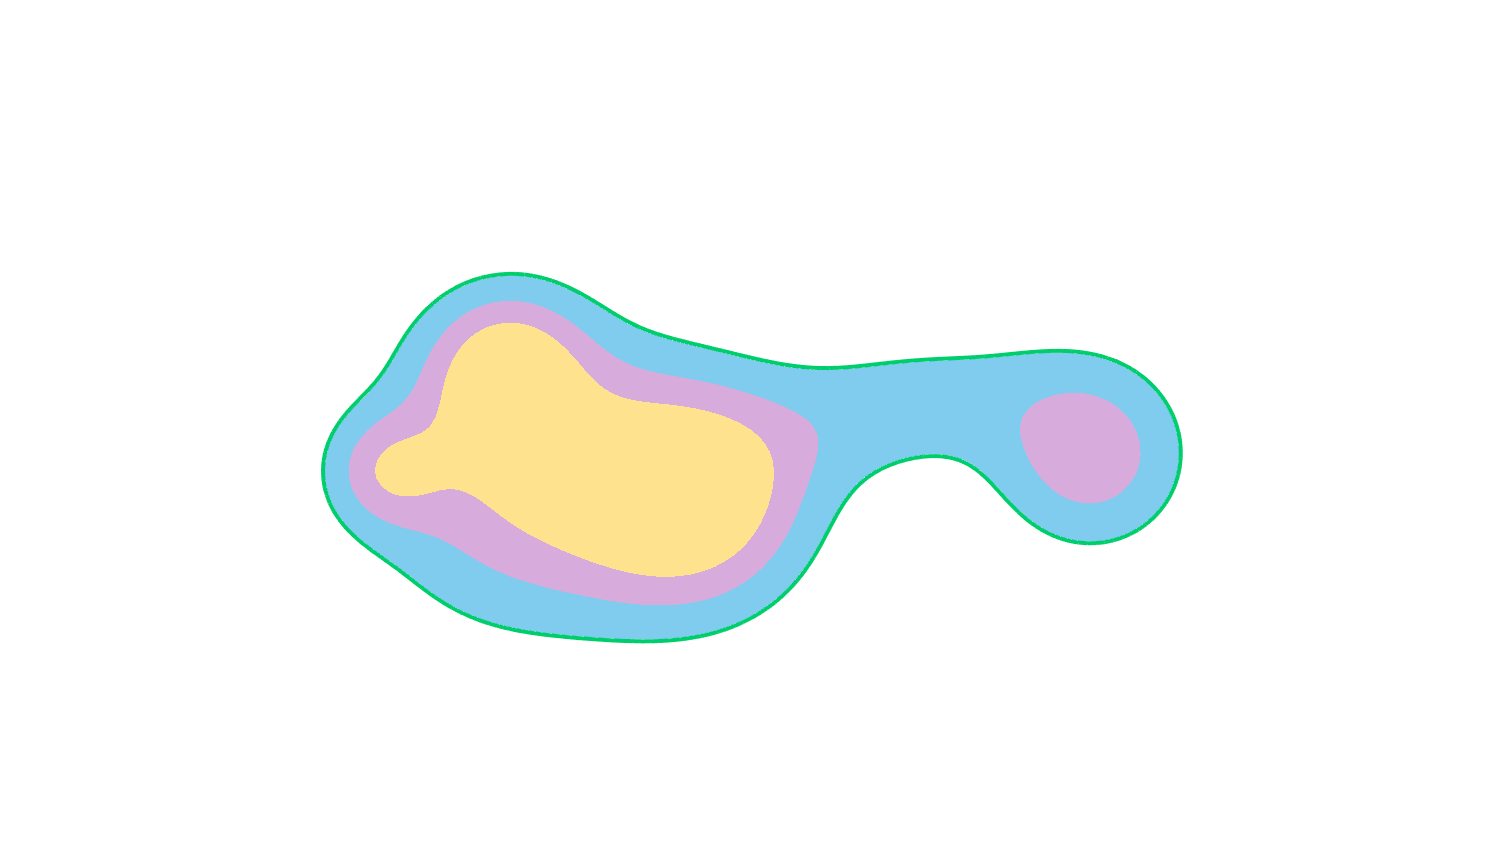
\includegraphics[trim=300 200 200 200, clip, width=0.3\textwidth]{../scripts/figures/surf/ass2_B_top.png}
  \end{textblock*}
\end{frame}


\begin{frame}
  \frametitle{{\small Assumption 2, Duality, and the Algorithmic TCC}}

  \begin{textblock*}{12cm}(0.5cm,2cm)
    \begin{small}
      \begin{itemize}
        \item Cannot compute the homology of offsets directly.
        \item Do not know $\mathbf{dim}~\hom_0(D\setminus B_\omega)$.
        \item Cannot compute the homology of complements directly.
      \end{itemize}
    \end{small}
  \end{textblock*}

  % \begin{itemize}
  %   \item Can't compute homology of complements: duality
  %   \item don't know number of connected components: assumption 2
  %   \item Rips-\v Cech interleaving and the Algorithmic TCC
  % \end{itemize}
  \begin{textblock*}{10cm}(1cm,5cm)
    \textbf{Duality:} $\hom_d(P^\e,Q^\e)\cong\hom_0(D\setminus Q^\e, D\setminus P^\e)$.\vspace{2ex}

  \end{textblock*}

  % \begin{textblock*}{12cm}(1cm,4.5cm)
  %
  % \end{textblock*}
\end{frame}


% %
% % \begin{frame}
% %   \frametitle{Overview: Main Theorems}
% %
% %   \begin{textblock*}{11cm}(1cm,2cm)
% %     \begin{small}\begin{theorem}[Geometric TCC]
% %         If
% %         \[ \mathbf{rk}~\hom_0((\overline{Q_1^\delta},\overline{P^\delta})\hookrightarrow (\overline{Q_0^\delta},\overline{P^\delta}))\geq \mathbf{dim}~\hom_0(D\setminus B_\omega)\]
% %         then $D\setminus B_\omega\subseteq P^\delta$ and $Q_0^\delta$ surrounds $P^\delta$ in $D$.
% %     \end{theorem}\end{small}
% %   \end{textblock*}
% %
% %   \begin{textblock*}{11cm}(1cm,5cm)
% %     \only<2>{\begin{small}\begin{theorem}[Algorithmic TCC]
% %         If
% %         \[ \mathbf{rk}~\hom_d(\rips^\delta(P,Q_0)\hookrightarrow \rips^{2\delta}(P, Q_1))\geq \mathbf{dim}~\hom_0(\rips^\delta(P\setminus Q_{0}))\]
% %         then $D\setminus B_\omega\subseteq P^\delta$ and $Q_0^\delta$ surrounds $P^\delta$ in $D$.
% %     \end{theorem}\end{small}}
% %   \end{textblock*}
% %
% % \end{frame}
%
%
% \begin{frame}
%   % \frametitle{{\small Setup and Notation}}
%   \frametitle{{\small Assumption 1 and the Geometric TCC}}
%
%   \begin{small}
%     Let $i : \hom_0(\overline{Q_1^\delta}, \overline{P^\delta})\to \hom_0(\overline{Q_0^\delta}, \overline{P^\delta})$.\vspace{1ex}
%
%     \begin{lemma}\label{lem:psurj}
%         If $B_\omega$ surrounds $D$ in $\X$ then $\mathbf{dim}~\hom_0(\overline{B_\omega}, \overline{D})\geq \mathbf{rk}~i$.
%     \end{lemma}\vspace{1ex}
%
%     Let $\ell : \hom_0(\overline{B_\omega}, \overline{D})\to \hom_0(\overline{Q_0^\delta}, \overline{P^\delta})$\vspace{1ex}
%
%     \begin{lemma}\label{lem:coverage}
%       If $\ell$ is injective then $D\setminus B_\omega\subseteq P^\delta$ and $Q_0^\delta$ surrounds $P^\delta$ in $D$.
%     \end{lemma}
%   \end{small}
%
%   % \begin{equation}\label{dgm:1}
%   % \begin{tikzcd}
%   %   (P^\delta, Q_{\omega-c\zeta}^\delta) \arrow[hookrightarrow]{r}\arrow[hookrightarrow]{d} &
%   %   (P^\delta, Q_{\omega+c\delta}^\delta) \arrow[hookrightarrow]{d} \\
%   %   %
%   %   (D, B_\omega) \arrow[hookrightarrow]{r} &
%   %   (D, B_{\omega+c(\delta+\zeta)}),
%   % \end{tikzcd}
%   % \begin{tikzcd}
%   %   \hom_0(\overline{B_{\omega+c(\delta+\zeta)}},\overline{D})\arrow{d}{m} \arrow{r}{j} &
%   %   \hom_0(\overline{B_\omega}, \overline{D}) \arrow{d}{\ell} \\
%   %   %
%   %   \hom_0(\overline{Q_{\omega+c\delta}^\delta}, \overline{P^\delta}) \arrow{r}{i} &
%   %   \hom_0(\overline{Q_{\omega-c\zeta}^\delta}, \overline{P^\delta}).
%   % \end{tikzcd}\end{equation}
% \end{frame}
%
% \begin{frame}
%   \frametitle{{\small Assumption 1 and the Geometric TCC}}
%
%   % \[\begin{tikzcd}
%   %   \hom_0(\overline{B_{\omega+c(\delta+\zeta)}},\overline{D})\arrow{d}{m} \arrow{r}{j} &
%   %   \hom_0(\overline{B_\omega}, \overline{D}) \arrow{d}{\ell} \\
%   %   %
%   %   \hom_0(\overline{Q_{\omega+c\delta}^\delta}, \overline{P^\delta}) \arrow{r}{i} &
%   %   \hom_0(\overline{Q_{\omega-c\zeta}^\delta}, \overline{P^\delta}).
%   % \end{tikzcd}\]
%
%   \begin{small}
%     Let $j: \hom_0(D\setminus B_{1})\to \hom_0(D\setminus B_\omega)$.\vspace{1ex}
%
%     \begin{theorem}[Geometric TCC]
%       % Let $j : \hom_0(\cmp{B_{\omega+c(\delta+\zeta)}},\cmp{D})\to \hom_0(\cmp{\B},\cmp{D})$ and $i : \hom_0(\cmp{\QQ^\of}, \cmp{P^\of})\to \hom_0(\cmp{\Q^\of}, \cmp{P^\of})$ be induced by inclusion.
%       %
%       If $j$ is surjective and $\mathbf{rk}~j\leq\mathbf{rk}~i$ then $\ell$ is injective. % $D\setminus B_\omega\subseteq P^\delta$ and $Q_{0}^\delta$ surrounds $P^\delta$ in $D$.
%     \end{theorem}\vspace{1ex}
%
%     If $j$ is surjective then $\mathbf{rk}~j\geq\mathbf{rk}~i$ so $\mathbf{rk}~j = \mathbf{rk}~i$.\vspace{1ex}
%
%     So $\mathbf{im}~j\cong \mathbf{im}~i \implies \ell$ is injective.
%   \end{small}
% \end{frame}
%

%
% \begin{frame}
%   \frametitle{{\small Assumption 2, Duality, and the Algorithmic TCC}}
%
%   \begin{small}
%     % \begin{theorem}[Algorithmic TCC]
%     %     If
%     %     \[ \mathbf{rk}~\hom_d(\rips^\delta(P,Q_0)\hookrightarrow \rips^{2\delta}(P, Q_1))\geq \mathbf{dim}~\hom_0(\rips^\delta(P\setminus Q_{0}))\]
%     %     then $D\setminus B_\omega\subseteq P^\delta$ and $Q_0^\delta$ surrounds $P^\delta$ in $D$.
%     % \end{theorem}\vspace{2ex}
%
%     Using duality $\mathbf{rk}~\hom_d((P^\delta, Q_0^\delta)\hookrightarrow (P^\delta, Q_1^\delta)) = \mathbf{rk}~i$\vspace{2ex}
%
%     $\mathbf{rk}~\hom_d(\cech^\delta(P, Q_0)\hookrightarrow \cech^\delta(P, Q_1))=\mathbf{rk}~i$ by the Nerve Theorem\vspace{2ex}
%
%     $\rips^\delta(P, Q_0)\subseteq\cech^\delta(P, Q_0)\subseteq\cech^\delta(P, Q_1)\subseteq\rips^{2\delta}(P, Q_1)$\vspace{2ex}
%
%     So $\mathbf{rk}~i\geq \mathbf{rk}~\hom_d(\rips^\delta(P,Q_0)\hookrightarrow \rips^{2\delta}(P, Q_1))$\vspace{2ex}
%
%     If $\hom_0(D\setminus B_\omega\hookrightarrow D\setminus B_{0})$ is injective then $\mathbf{dim}~\hom_0(\rips^\delta(P\setminus Q_{0})) \geq \mathbf{dim}~\hom_0(D\setminus B_\omega)$.
%   \end{small}
% \end{frame}
%
% % \begin{frame}
% %   \frametitle{{\small Duality, Assumption 2, and the Algorithmic TCC}}
% %
% %   % \begin{itemize}
% %   %   \item Can't compute homology of complements: duality
% %   %   \item don't know number of connected components: assumption 2
% %   %   \item Rips-\v Cech interleaving and the Algorithmic TCC
% %   % \end{itemize}
% %   \begin{small}
% %     \[ \hom_k(\rips^\e(P, Q))\xrightarrow{J}\hom_k(\cech^\e(P, Q))\xrightarrow{I}\hom_k(\rips^\e(P, Q))\]
% %     % so
% %     % \[\mathbf{rk}~\hom_d(\cech^{\delta}(P, Q_{\omega-c\zeta})\hookrightarrow\cech^{\delta}(P, Q_{\omega+c\delta})) \geq\mathbf{rk}~ \hom_d(\rips^{\delta}(P, Q_{\omega-c\zeta})\hookrightarrow\rips^{2\delta}(P, Q_{\omega+c\delta}))\]
% %
% %     % \begin{theorem}[Algorithmic TCC]\label{thm:algo_tcc}
% %     %   Suppose $\hom_0(D\setminus B_{\omega+c(\delta+\zeta)}\hookrightarrow D\setminus B_\omega)$ is surjective and $\hom_0(D\setminus B_\omega\hookrightarrow D\setminus B_{\omega-c(\delta+\zeta)})$ is injective.
% %     %
% %     %    If $\mathbf{rk}~\hom_d(\rips^\delta(P, Q_{\omega -c\zeta})\hookrightarrow \rips^{2\delta}(P, Q_{\omega+c\delta})) \geq \mathbf{dim}~\hom_0(\rips^\delta(P\setminus Q_{\omega-c\zeta}))$ then $D\setminus B_\omega\subseteq P^\delta$ and $Q_{\omega-c\zeta}^\delta$ surrounds $P^\delta$ in $D$.
% %     % \end{theorem}
% %
% %     \begin{theorem}[Algorithmic TCC]\label{thm:algo_tcc}
% %       Suppose $\hom_0(D\setminus B_{1}\hookrightarrow D\setminus B_\omega)$ is surjective and $\hom_0(D\setminus B_\omega\hookrightarrow D\setminus B_{0})$ is injective.
% %
% %        If $\mathbf{rk}~\hom_d(\rips^\delta(P, Q_{0})\hookrightarrow \rips^{2\delta}(P, Q_{1})) \geq \mathbf{dim}~\hom_0(\rips^\delta(P\setminus Q_{0}))$ then $D\setminus B_\omega\subseteq P^\delta$ and $Q_{0}^\delta$ surrounds $P^\delta$ in $D$.
% %     \end{theorem}
% %   \end{small}
% %
% %   % \begin{textblock*}{12cm}(1cm,4.5cm)
% %   %
% %   % \end{textblock*}
% % \end{frame}
